\documentclass[12pt, a4paper]{article}

\usepackage[utf8]{inputenc}
\usepackage[hmargin=2.5cm,vmargin=2.5cm]{geometry}
\usepackage[brazil]{babel}
\usepackage{graphicx}
\usepackage{amsmath}
\usepackage{steinmetz}
\usepackage{float}
\usepackage{graphicx}

\title{Relatório 4\\Exercício Prático \textit{PSpice}}
\author{Gustavo Ciotto Pinton - 117136}
\date{Abril 2013}

\begin{document}

    {\large
    \centerline{Exercício Prático 4}
    \centerline{Gustavo Ciotto Pinton 117136}
    }
    \section*{Questões}
    
    \begin{enumerate}
    
    
        \item Considere o circuito diferencial da figura \ref{circ41} na seção \textbf{Anexos}. Inicialmente, vamos determinar os valores das resistências \(R_C\) ligadas ao pinos coletores de \(Q_1\) e \(Q_2\). Para tal, considere que os valores de \(\beta\) dos transistores são iguais e que seus valores são 220\footnote{Valor obtido observando-se o modelo utilizado pelo \textit{PSpice}}. Considere também uma fonte de corrente DC \(I=1.136mA\), as baterias de \(V_{CC}\) e \(-V_{CC}\) e as seguintes equações, supondo que os transistores trabalhem no modo ativo.
        
        A primeira expressão relaciona as correntes de coletor e emissor, de forma que        
        \begin{equation} \label{eq:ieic}
        I_C = \frac{\beta}{\beta+1} I_E = \alpha I_E \approx 0.996 I_E
        \end{equation}
                
        Voltando ao circuito, facilmente se vê, por inspeção, que 
        
        \[I_{E1} = I_{E2} = \frac{I}{2}\ = 568 \mu A \]
        
        Sendo assim, através da relação \ref{eq:ieic}, chega-se a \[I_{C1} = \alpha I_{E1} = \alpha \frac{I}{2} = 0.996 \frac{1.136mA}{2} = 565.43 \mu A\] e, da mesma forma, \[I_{C2} = \alpha I_{E2} = \alpha \frac{I}{2} = 0.996 \frac{1.136mA}{2} = 565.43 \mu A \]
        
        Finalmente, o valor de \(R_C\) pode ser calculado através da equação:
        
        \begin{equation} \label{eq:rc}
        R_C = \frac{V_{CC}-V_D}{I_C}
        \end{equation}
        
        Substituindo os valores em \ref{eq:rc} e calculando \(V_C\) para aproximadamente a metade da excursão máxima possível, isto é, \(V_C = 5V\), obtém-se \(R_C=8.843k \Omega \). 

        As demais voltagens são:
        \[V_{B1} = V_{B2} = 0\]
        \[V_{E1} = V_{E2} = V_B - V_{BE} \approx 0 - 0.7 = -0.7V\]

        A transcondutância \(g_m\) é
        
        \begin{equation} \label{eq:gm}
        g_m \approx 40I_C \approx 0.02262 \Omega ^{-1}
        \end{equation}
        
        A análise de polarização (BIAS POINT DETAIL) nos fornece as tabelas \ref{table:tabelaVoltagemBIAS} e \ref{table:tabelaCorrenteBIAS}. Comparando os dados simulados com os teóricos, conclui-se que os teóricos adequam-se com grande precisão, com excessão das tensões \(V_E\) nos pinos de emissor. O motivo dessa diferença é que, nas análises, consideramos \(V_{BE} = 0.7V\), sendo que o modelo utilizado pelo programa tal valor é \(V'_{BE} = 0.6117V\).
        
        \begin{table} [h!]
            \caption{Voltagens de polarização. }
            \centering
            \label{table:tabelaVoltagemBIAS}
            
                \begin{tabular}{ c | c | c | c } 
        
                NODE & VOLTAGE [V] & NODE & VOLTAGE [V] \\
                \hline
                \(V_{C1}\) & 5.0006 & \(V_{C2}\) & 5.0006 \\
                \(V_{CC}\) & 10.0000 & \(-V_{CC}\) & -10.0000 \\
                \(V_{E1}\) & -0.6117 & \(V_{E2}\) & -0.6117\\
                \(V_{B1}\) & 0.0000 & \(V_{B2}\) & 0.0000\\
                
                \end{tabular}
       \end{table}  
       
       \begin{table} [h!]
            \caption{Correntes de polarização. }
            \centering
            \label{table:tabelaCorrenteBIAS}
            
                \begin{tabular}{ c | c | c | c } 
        
                NODE & CURRENT [A] & NODE & CURRENT [A] \\
                \hline
                \(I_{C1}\) & 5.65E-04 & \(I_{C2}\) & 5.65E-04 \\
                \(I_{B1}\) & 2.65E-06 & \(I_{B2}\) & 2.65E-06\\
                \(I_{E1}\) & 5.68E-04 & \(I_{E2}\) & 5.68E-04\\
                
                \end{tabular}
       \end{table} 
        
      
    Vamos agora analisar o circuito de maneira AC. O primeiro passo é determinar a corrente \(i_e\), que é a corrente que sai do emissor do transistor \(Q_1\), cujo valor é obtido através da equação \ref{eq:ie}.
    
    \begin{equation} \label{eq:ie}
    i_e = \frac{v_i}{2r_e}    
    \end{equation}
    
    O segundo passo é determinar as voltagens nos pinos coletores de cada transistor. Para isso, leva-se em consideração que \(i_e = i_{e1} = -i_{e2}\), \( i_{c1} = - i_{c2} = \alpha i_{e1}\) e \(r_e = \frac{\alpha}{g_m}\ = 44.01 \Omega \). Sendo assim, obtém-se
    
    \[ v_{c1} = -R_C \alpha i_{e1} = - \frac{R_C}{2r_e} \alpha v_i \]
    e
    \[ v_{c2} = -R_C \alpha i_{e2} = \frac{R_C}{2r_e} \alpha v_i \]
    
    O ganho diferencial é, portanto
    
    \begin{equation} \label{eq:gDif}
    A_d = \frac{v_{c2} - v_{c1}}{v_i} = 2\alpha \frac{R_C}{2r_e} = \alpha \frac{R_C}{r_e} = 200.0 \frac{V}{V}
    \end{equation}
    
    e os não diferenciais, quando a saída é a tensão do pino coletor de \(Q_1\) e quando é no pino de \(Q_2\), respectivamente,
    
    \[ A_{nd1} = \frac{v_{c1}}{v_i} = -\frac{\alpha R_C}{2r_e} = -100.0 \frac{V}{V} \]
    e
    \[ A_{nd2} = \frac{v_{c2}}{v_i} = \frac{\alpha R_C}{2r_e} = 100.0 \frac{V}{V} \]
    
    
    Considere agora o gráfico da figura \ref{ondavc1} da seção \textbf{Anexos} que corresponde ao transitório da tensão \(v_{C1}\). Como esperado, o sinal de saída está oscilando em torno de 5V, que é justamente a tensão de polarização. Quando \(v_i\) atinge o seu pico positivo, a onda de saída atinge o negativo, justificando o sinal negativo em \(A_{nd1}\), e com amplitude, em relação a 5V, de aproximadamente a \(\pm 0.9V\). Levando em consideração que o valor teórico calculado foi \(100*0.10 mV = 1V\), os resultados obtidos apresentaram um erro de 10\% em relação à teoria. Uma das possíveis causas é que, no cálculo de \(g_m\), utilizamos \(V_T = 25mV\), sendo que não sabe-se ao certo que valor o \textit{PSpice} usa.
    
    O mesmo raciocínio pode ser utilizado no gráfico da figura \ref{ondavc2} que corresponde ao transitório da tensão \(v_{C2}\). Da mesma maneira que \(v_{C1}\), a onda oscila em torno de 5V. A diferença é que quando \(v_i\) atinge o seu pico positivo, a onda de saída também atinge o positivo, ao contrário do caso passado. Isso era esperado, visto que não existe um sinal negativo na expressão de \(A_{nd2}\). O erro na amplitude também é próximo de 10\% e a causa é a mesma já explicada anteriormente.
    
    Nas análises realizadas anteriormente, assumimos que os transitores estavam operando em modo ativo, isto é, EBJ diretamente polarizada e CBJ reversamente. Isto era facilmente garantido pelo valor escolhido da tensão de polarização - aproximadamente metade da excursão máxima - e pelo fato que a entrada eram sinais de pequenas amplitudes. Considere agora uma tensão de entrada com um pico relativamente alto, com \(v_i = 1V\). Para tensões do coletor maiores ou iguais a \(V_{CC}=10V\), a junção CBJ estará diretamente polarizada e o transistor trabalhará em modo saturado. Por outro lado, se a tensão no coletor for suficientemente baixa (\(v_C \le V_{BCon} \approx 0.5V \)), o transistor não conduzirá corrente e estará cortado, uma vez as duas junções estarão reversamente polarizadas. 
    
    O gráfico da figura \ref{ondavc1satcutoff} da seção \textbf{Anexos} representa este caso para a onda de saída em \(v_{C1}\). Como o ganho \(A_{nd1}\) é negativo, se \(v_i \ge 0.05V\), então \(v_{c1} = A_{nd1}v_i \le -5V\) e, portanto, \(v_{C1} = V_{C1} + v_{c1} \le 0\). Neste intervalo de valores, o transistor \(Q_1\) estará cortado. Considere agora a situação em que \(v_i \le -0.05V\): \(v_{c1} = A_{nd1}v_i \ge 5V\) e \(v_{C1} = V_{C1} + v_{c1} \ge V_{CC} = 10V\), resultando \(Q_1\) em estado em estado de saturação. Como esperado, o gráfico adquire um aspecto linear nesta faixa, cuja tensão de saída não muda. Finalmente, o transistor \(Q1\) só operará em estado ativo no intervalo próximo de \((-0.05V , 0.05V)\).
    
    Podemos repetir o raciocínio para \(Q_2\), obtendo o gráfico da figura \ref{ondavc2satcutoff}. Os resultados são similares, mas com a ressalva que o sinal do ganho será invertido e, assim, no intervalo de tensões em que \(Q_1\) estaria cortado, \(Q_2\) estaria saturado e vice-versa.
    
    A figura \ref{ondavdcutoff}, que é o transitório da tensão diferencial, resume a situação: o amplificador só estará funcionando entre -10V e 10V. 
    
    Analisemos agora as frequências de corte inferior e superior. A inferior é calculada através dos valores dos capacitores que foram incorporados ao circuito e, neste caso, como tais capacitores não estão presentes, \(f_L\) não existe. Em outras palavras, este amplificador trabalha mesmo para pequenas frequências, desde \(0Hz\). A superior, por outro lado, é determinada por capacitâncias internas aos próprios transitores. A frequência superior pode ser calculada através da equação:
    
    \begin{equation} \label{eq:freq}
    f_H = \frac{1}{2 \pi C_{in} R'_{sig}} 
    \end{equation}
    
    em que 
    
    \begin{equation}
    C_{in} = C_{\pi } + C_{\mu }(1+ g_m R'_L)
    \end{equation}
    
    e
    
    \begin{equation}
    R'_{sig} = r_{\pi } || [ r_x + (R_B||R_{sig}) ]
    \end{equation}
        
    
    \(C_{\pi } = 48.10 pF\) e \(C_{\mu } = 3.69 pF\) são obtidos através da observação de \textit{Examine Output}, e \(R'_L = R_C||r_o = 8.843k || 189k = 8.447k \Omega \). Considerando que \( r_x = 1,3 \Omega \) (da mesma forma, através do arquivo gerado por \textit{Examine Output}) e que \(R_B = R_{sig} = 0\), calcula-se 
    
    \begin{equation} \label{eq:rpi}
    r_{\pi } = \frac{\beta}{gm} = 9.727k\Omega
    \end{equation}
    
    \[R'_{sig} \approx r_{\pi } || r_x = \frac{\frac{\beta}{gm} r_x}{r_x + \frac{\beta }{g_m}} = 1.29 \Omega \]
    
    e 
    \[C_{in} = C_{\pi } + C_{\mu }(1+ g_m R'_{L}) =  15.2nF\]
    
    Finalmente, substituindo os valores em \ref{eq:freq}, obtem-se
    
    \[f_H = \frac{1}{2\pi *15.2*1.29*10^{-9}} = 8.12MHz \]
    
    O resultado obtido para o ganho diferencial está representando na figura \ref{graf411}. O ganho de tensão diferencial obtido pelo gráfico foi aproxidamente \[A'_d = \frac{v'_o}{v_i} \approx \frac{1.83}{0.01} \approx 183 \frac{V}{V}\] sendo que o calculado pela equação \ref{eq:gDif} foi \(A_d = 200.0\). A diferença de \(8.5 \% \) pode ser explicada por algumas suposições e simplificações realizadas, como por exemplo, \(V_T = 25mV\) ou \(g_m \approx 40I_C \). 
    
    A frequência em que o ganho corresponde a sua metade, ou seja, \(A_d \approx 91.5\), é estimada em \(f'_H \approx 8.864MHz\), apresentando um erro de \(8\% \) em relação ao teórico. Tal erro deve-se principalmente aos diferentes parâmetros usados, como, por exemplo, a transcondutância (\(g_m\)) e, novamente, \(V_T\).
    
    A resistência de saída é definida como o valor de \(R_L\) que reduz o ganho à metade. Para calcula-la, coloca-se uma resistência entre os terminais da saída, como indicado na figura \ref{circ412}.
    Se efetuarmos essa mudança no circuito e simularmos novamente, obteremos o gráfico da figura \ref{graf412}, cujo ganho é \[A'_{\frac{d}{2}} \approx \frac{0.915}{0.010} \approx 91.5\]
    
    Como esperado este ganho é aproximadamente metade de \(A'_d \approx 183 \) e, portanto, \(R_{out} = 16.9k\Omega \) é um valor razoável para a resistência de saída.
    
    Finalmente, utilizando a ferramenta \textit{BJT MODEL PARAMETERS}, obtem-se a tabela \ref{table:bjtparam}.
    
    \begin{table} [h!]
            \caption{Parâmetros dos transistores BJT. }
            \centering
            \label{table:bjtparam}
            
                \begin{tabular}{ c | c | c | c } 
        
                PARAM & VALUE & PARAM & VALUE \\
                \hline
                \(I_{S}\) & 30.6E-15 A & \(I_{B}\) & 2.65E-06 A \\
                \(\beta \) & 220 & \(V_{BE}\) & 6.12E-01 V \\
                \(I_{C}\) & 5.65E-04 A & \(V_{CE}\) & 5.61E+00 V\\
                \(g_m \) & 2.18E-02 & \(r_{\pi }\) & 9.93E+03 \(\Omega\) \\
                \(f_{T}\) & 6.69E+07 Hz & \(r_{o}\) & 1.89E+05 \(\Omega\)\\
                \end{tabular}
       \end{table}
    
    
    Através das equações \ref{eq:gm} e \ref{eq:rpi}, obtemos, respectivamente, \(g_m = 0.02262 \Omega^{-1}\) e \(r_{\pi} = 9.727k\Omega\). Comparando com os valores da tabela \ref{table:bjtparam}, podemos concluir que os resultados foram muito próximos, com erros de \(3\% \) para a transcondutância e \( 2 \% \) para \(r_{\pi }\), causados, novamente, pelas suposições feitas.
    
    
    
    
    
    \item Seja agora o circuito da figura \ref{circ42} que representa um estágio de saída CLASSE B. Considere \(R_L = 10.136 \Omega \) e \(v_i\) uma fonte de tensão senoidal de amplitude 10V.
    
    Vamos analisar a função de transferência deste circuito através da ferramenta \textit{DC Sweep}, obtendo a saída para valores de \(v_i\) entre -10V e 10V, variando 0.1. O resultado desta simulação encontra-se na figura \ref{graf421} da seção \textbf{Anexos}. Nesta figura, percebe-se que existe uma região em que \(v_o = 0\), chamada de \textit{crossover distortion}. Para entender esta característica, temos que estudar comportamento de cada transistor. Considere \(Q_1\) inicialmente: se \(v_i \le V_{BCon} \approx 0.5V\), \(Q_1\) não conduz e está cortado. Seja \(Q_2\) agora: se \(v_i \ge V_{BCon} \approx -0.5V\), \(Q_2\) não conduz e está cortado. Portanto, na faixa de valores entre -0.5V e 0.5V, ambos os transistores estão cortados e a saída é 0. Esta análise também nos revela que quando \(Q_1\) está conduzindo (lado direito do gráfico), \(Q_2\) está cortado e vice-versa.
    
    Realizada a análise DC, vamos nos concentrar na parte AC. Vamos considerar que a tensão de saída é aproximadamente igual a de entrada, uma vez que a tensão de junção EBJ \(\approx 0.7V\) é muito menor que 10V.  Tem-se, portanto:
    
    \begin{equation}
    v_o = v_i - V_{BE} \approx v_i = V_o \sin (wt)
    \end{equation}
    
    A corrente na carga pode ser escrita por 
    
    \begin{equation}
    i_l = \frac{V_o}{R_L} \sin (wt)
    \end{equation}
    
    A potência instantânea e média (ou eficaz) na carga são calculadas, respectivamente,  através de 
    
    \begin{equation}
    P_L (t) = v_o i_l = \frac{V_o^2}{R_L} \sin ^2 (wt)
    \label{eq:potins}
    \end{equation}
    
    \begin{equation}
    \overline{P_L} = \frac{1}{2}\frac{V_o^2}{R_L}
    \label{eq:potLmed}
    \end{equation}
     
    Utilizando os valores \(R_L = 10.136 \Omega \) e \(V_o = 10V\) em \ref{eq:potLmed}, obtem-se \(\overline{P_L} = 4.933W\). Vamos considerar nesta etapa os gráficos \ref{graf422V} e \ref{graf422I}, obtidos através das análises dos transitórios da tensão e corrente, respectivamente, na carga. A tensão de saída apresenta um amplitude de aproximadamente \(V'_o \approx 9.2V\) e a corrente, um pico de \(I'_o \approx 0.92A\). Utilizando a expressão \ref{eq:potLmed}, calcula-se uma potência média \(\overline{P'_L} = 4.232W\). O erro de \(\approx 16\% \) entre as potências teórica e prática pode ser explicado pelas simplificações realizadas, como a suposição de que a \textit{crossover distortion} não afetava as contas e inexistência de \(V_{BE}\) nas equações.
    
    A potência média utilizada nas fontes de tensão é escrita pela equação
    
    \begin{equation}
    \overline{P_S} = \frac{2}{\pi } \frac{V_o}{R_L}V_{CC}
    \label{eq:psmed}
    \end{equation}
    
    Substituindo os valores em \ref{eq:psmed}, obtem-se \(\overline{P_S} =
    6.281W\). Repetindo o método utilizado para calcular a potência na carga, simulamos os transitórios das correntes nas duas fontes de tensão. Como cada transistor trabalha sem a interferência do outro, isto é, se \(Q_1\) está conduzindo, então \(Q_2\) está cortado e vice-versa, a corrente que passa por cada fonte é uma metade da total e corresponde a um semi-ciclo  (pela bateria positiva flui a corrente positiva e pela negativa, evidentemente, o restante). É por essa razão que existe o fator \(\frac{1}{\pi }\) na fórmula \ref{eq:psmed},  sendo o resultado da média de uma função senoidal com apenas um ciclo.
    
    Os transitórios das correntes nas baterias positivas e negativas estão, respectivamente, representadas nas figuras \ref{graf423I+} e \ref{graf423I-}. As amplitudes são \(I^+ = 0.9A\) e \(I^- = -0.88A\). As potências eficazes são \(\overline{P'_+} = V_{CC}\frac{I^+}{\pi } = 2.865W\) e \(\overline{P'_-} = V_{CC}\frac{I^-}{\pi } = 2.801W\) e a total é \(\overline{P'_S}= \overline{P'_-} + \overline{P'_+} = 5.667W\). O erro de \(\approx 9.8 \% \) entre os resultados prático e teórica podem ser explicados pelos mesmos motivos do caso anterior.
    
    A eficiência do amplificador é definida por 
    
    \begin{equation}
    \eta = \frac{\overline{P_L}}{\overline{P_S}}
    \end{equation}
    
    A eficiência teórica, como esperava-se, é máxima quando \(V_o = V_{CC}\) e vale \[\eta = \frac{\overline{P_L}}{\overline{P_S}} = \frac{4.933}{6.281} = 78.5 \% \] e a obtida experimentalmente é \[\eta '= \frac{\overline{P'_L}}{\overline{P'_S}} = \frac{4.232}{5.667} = 74.7 \% \]
    
    com um erro de \(\approx 5 \% \). 
    \end{enumerate}
    
    \newpage
    \section*{Anexos}
    
    \begin{figure}[h!] 
        \centering
        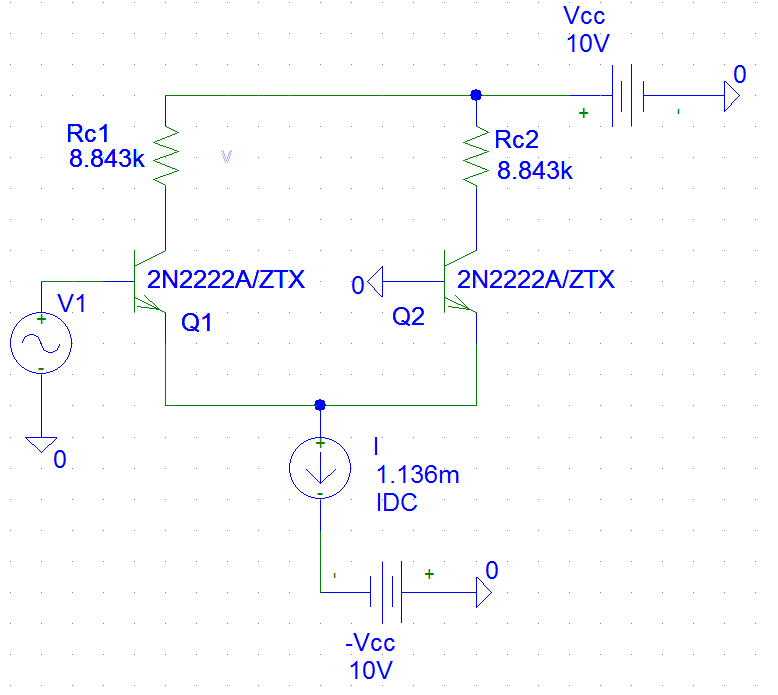
\includegraphics[width=0.40\textheight]{circ41}
        \caption{Circuito diferencial BJT.}        
        \label{circ41}
    \end{figure}
    
    \begin{figure}[h!] 
        \centering
        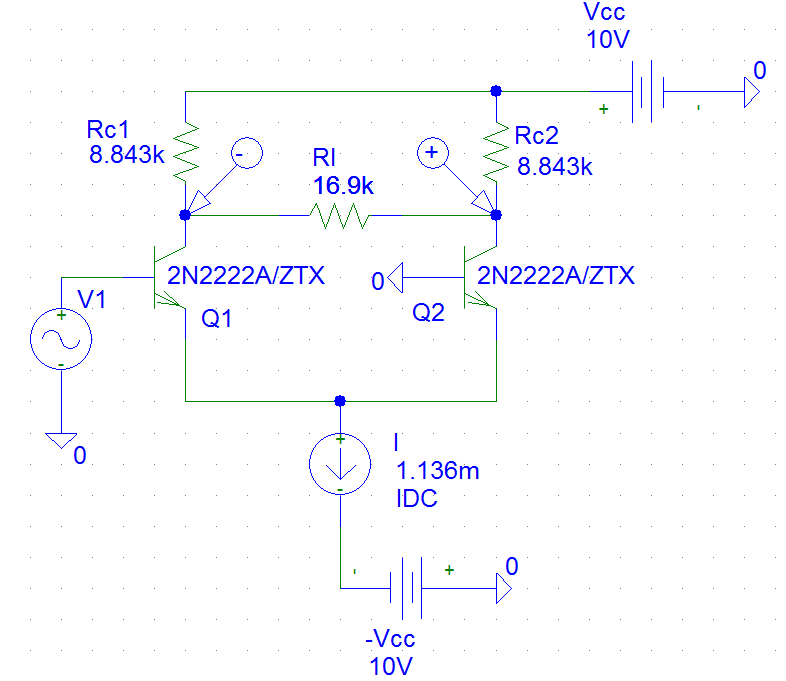
\includegraphics[width=0.40\textheight]{circ412}
        \caption{Circuito diferencial BJT com resistência \(R_L\).}        
        \label{circ412}
    \end{figure}
    

    \newpage
    
    
    \begin{figure}[h!] 
        \centering
        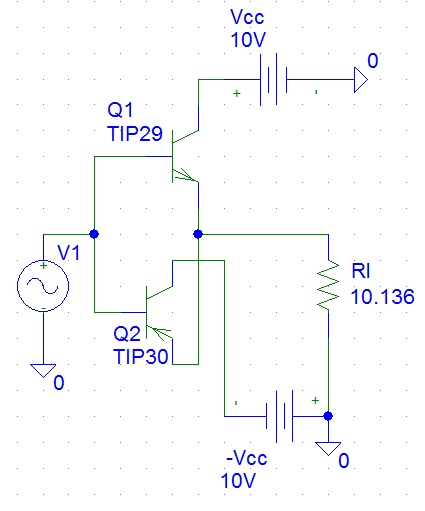
\includegraphics[width=0.40\textheight]{circ42}
        \caption{Estágio de saída CLASSE B.}        
        \label{circ42}
    \end{figure}
    

    \newpage
    
    \begin{figure}[h!] 
        \centering
        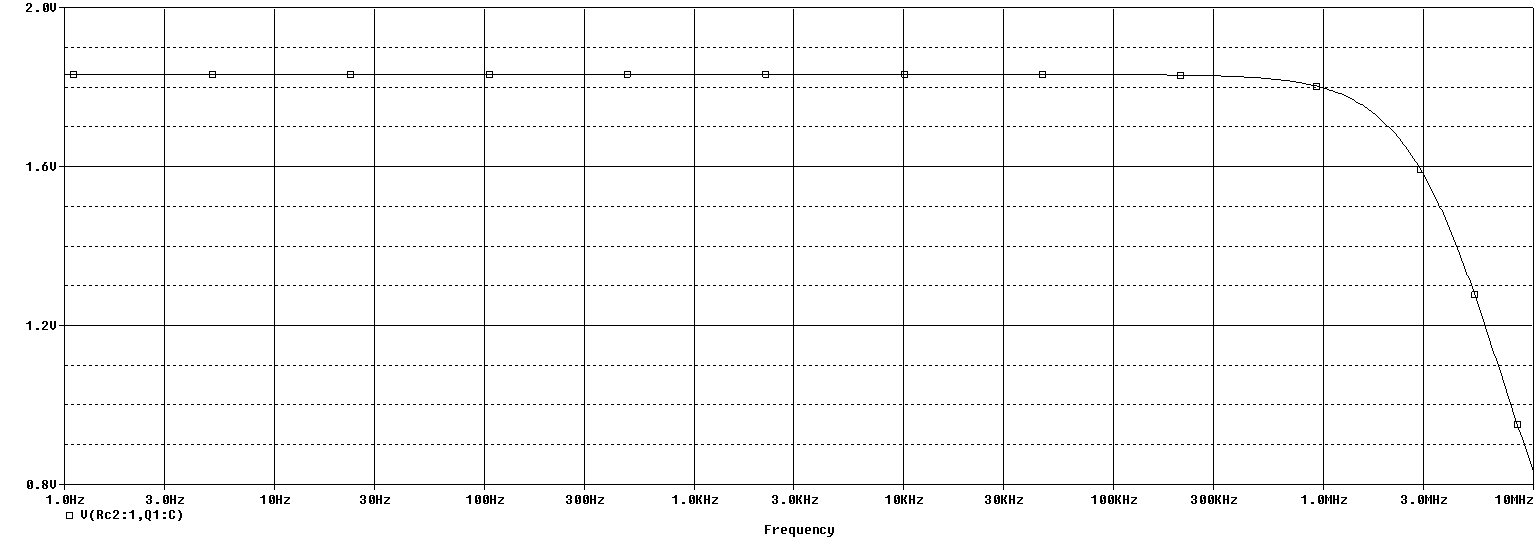
\includegraphics[width=1\textheight, angle=-90]{graf411}
        \caption{Função de transferência diferencial.}        
        \label{graf411}
    \end{figure}
    
    \newpage
    
    \begin{figure}[h!] 
        \centering
        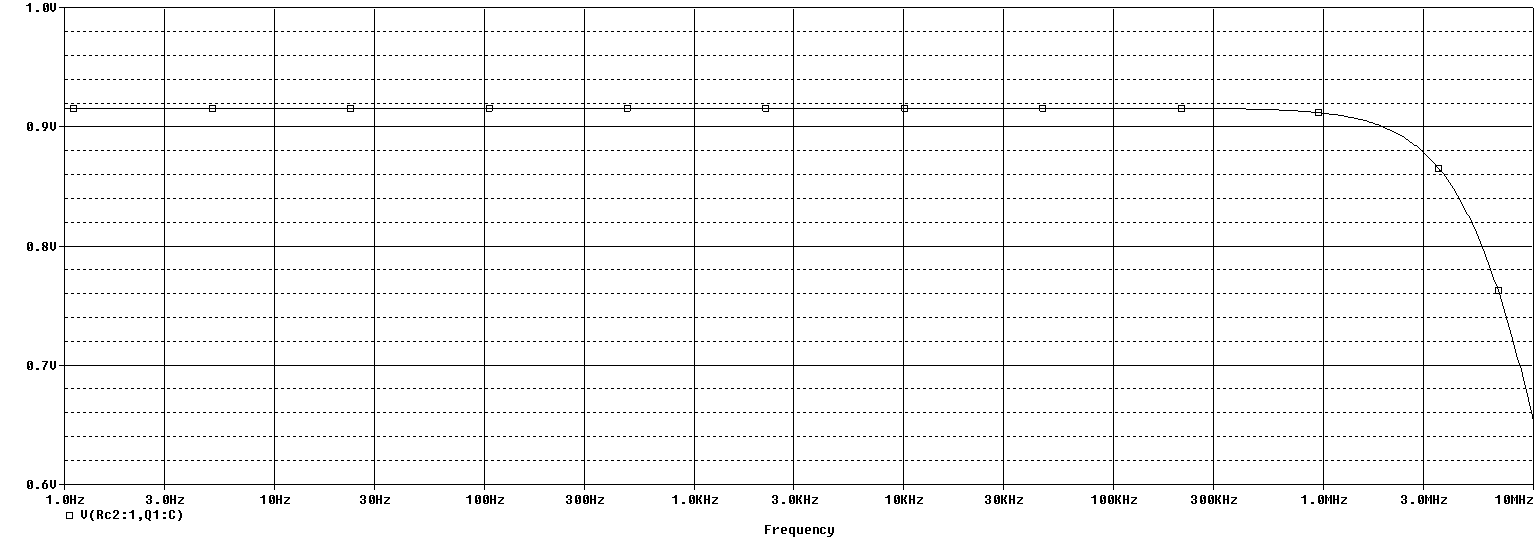
\includegraphics[width=1\textheight, angle=-90]{graf412}
        \caption{Função de transferência diferencial reduzido à metade.}        
        \label{graf412}
    \end{figure}

    \newpage
    
    \begin{figure}[h!] 
        \centering
        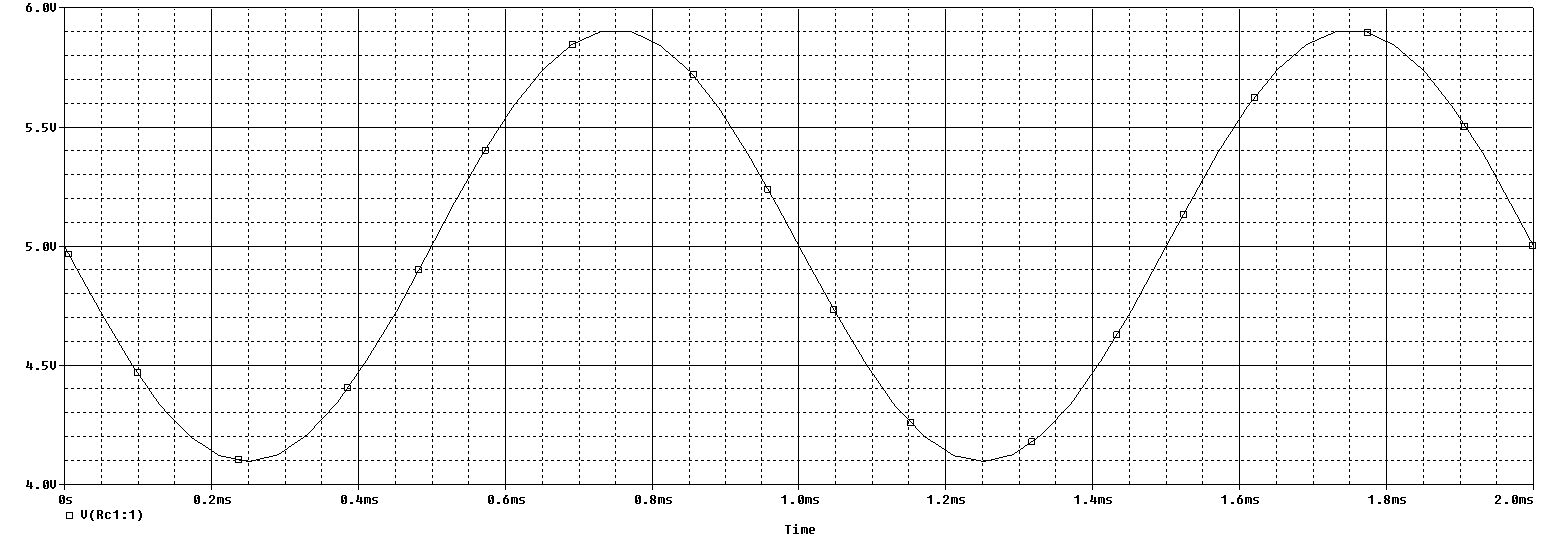
\includegraphics[width=1\textheight, angle=-90]{ondavc1}
        \caption{Transiente de onda de saída de \(v_{C1}\).}        
        \label{ondavc1}
    \end{figure}
    
    \newpage
    
    \begin{figure}[h!] 
        \centering
        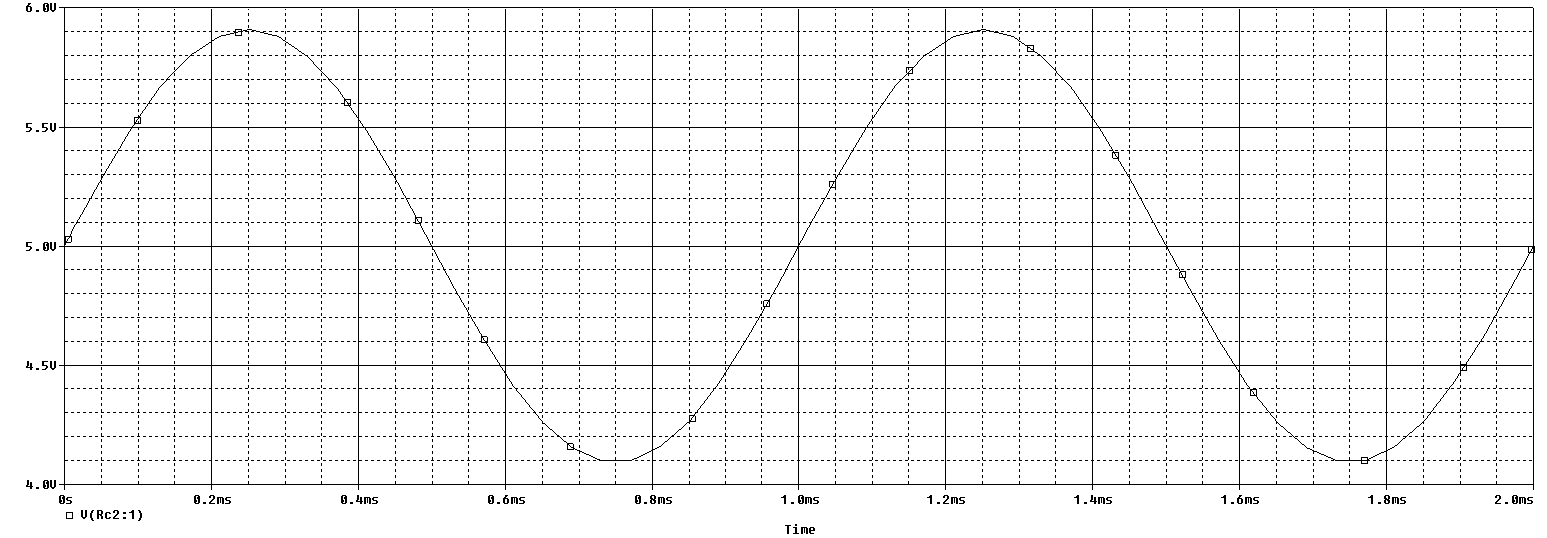
\includegraphics[width=1\textheight, angle=-90]{ondavc2}
        \caption{Transiente de onda de saída de \(v_{C2}\).}        
        \label{ondavc2}
    \end{figure}
    
    \newpage
    
    \begin{figure}[h!] 
        \centering
        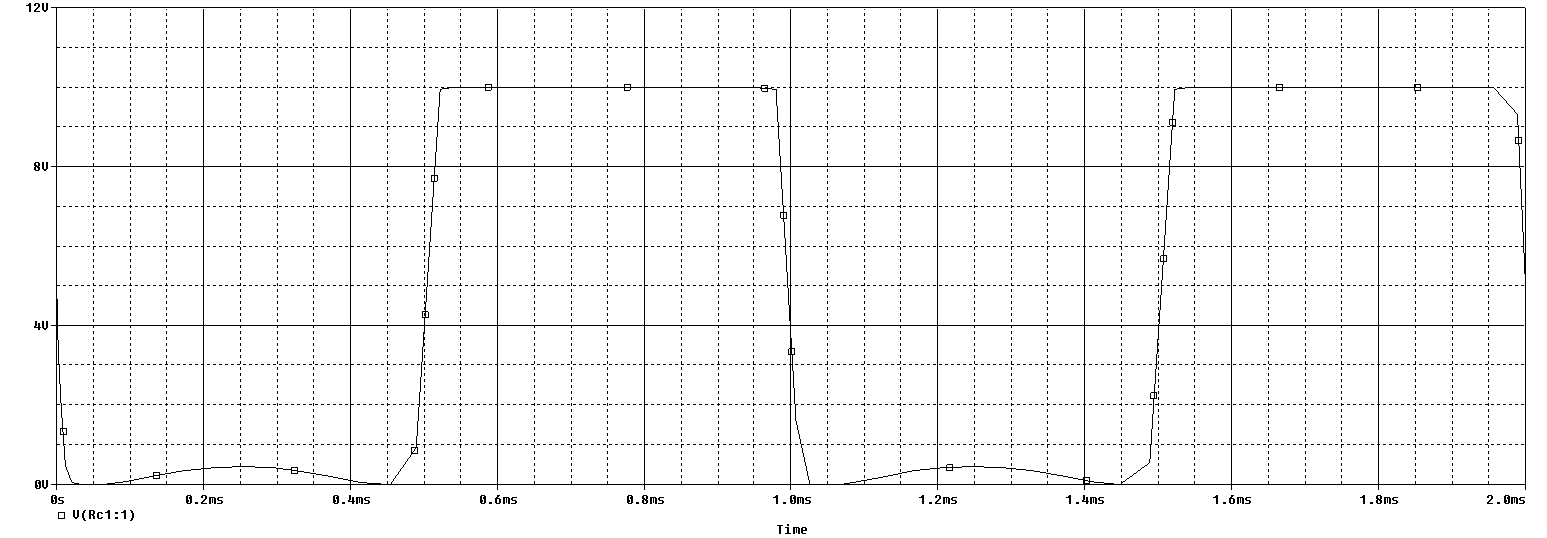
\includegraphics[width=1\textheight, angle=-90]{ondavc1satcutoff}
        \caption{Transiente de onda de saída de \(v_{C1}\) para \(v_i = 1V\).}        
        \label{ondavc1satcutoff}
    \end{figure}
    
    \newpage
    
    \begin{figure}[h!] 
        \centering
        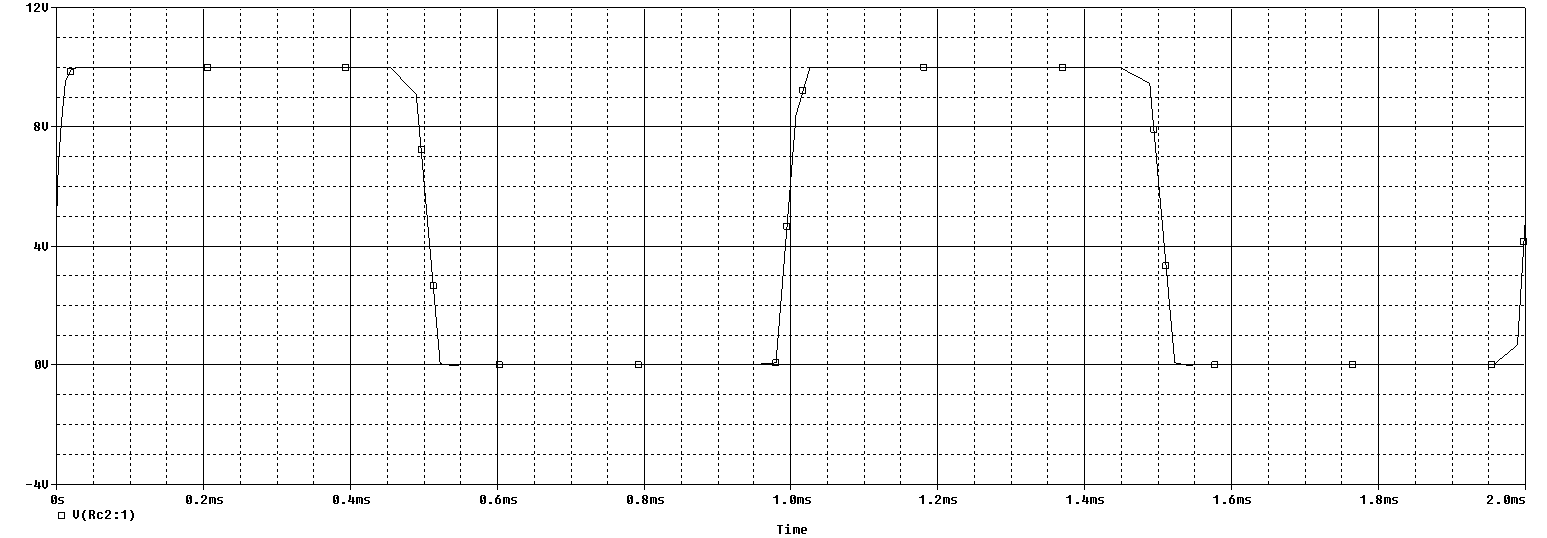
\includegraphics[width=1\textheight, angle=-90]{ondavc2satcutoff}
        \caption{Transiente de onda de saída de \(v_{C2}\) para \(v_i = 1V\).}        
        \label{ondavc2satcutoff}
    \end{figure}
    
    \newpage
    
    \begin{figure}[h!] 
        \centering
        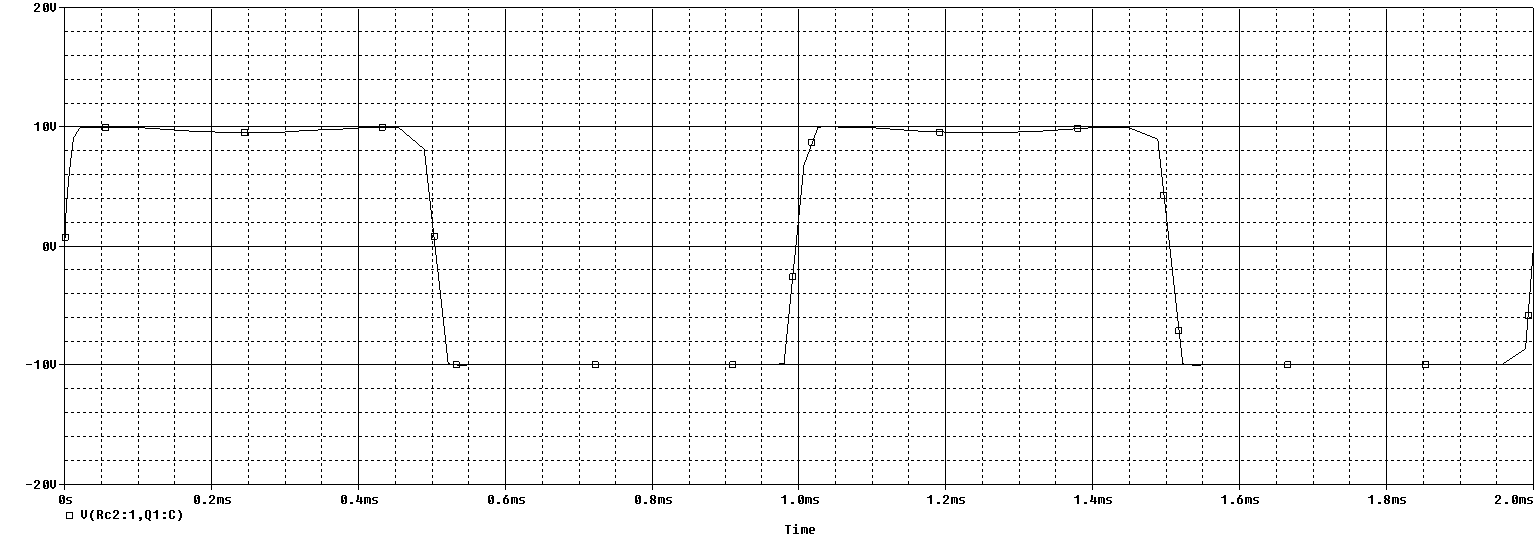
\includegraphics[width=1\textheight, angle=-90]{ondavdcutoff}
        \caption{Transiente de onda de saída de \(v_{d}\) para \(v_i = 1V\).}        
        \label{ondavdcutoff}
    \end{figure}
    
    \newpage
    
    \begin{figure}[h!] 
        \centering
        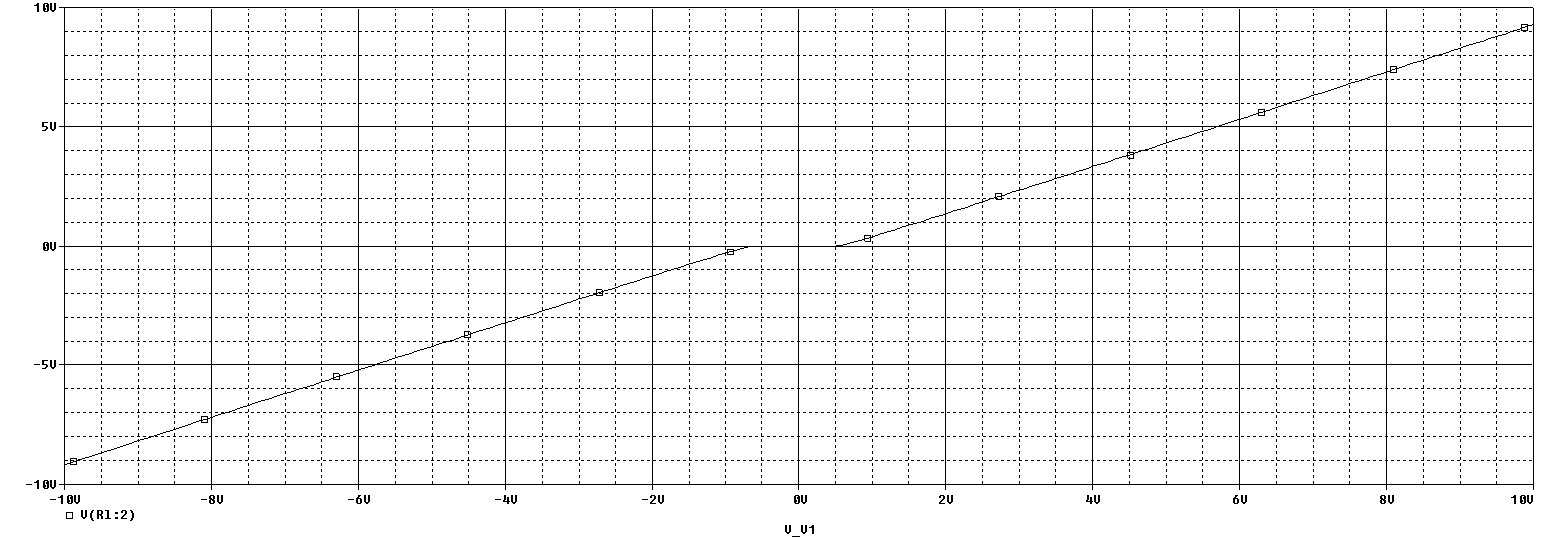
\includegraphics[width=1\textheight, angle=-90]{graf421}
        \caption{Função de transferência do circuito CLASSE B.}        
        \label{graf421}
    \end{figure}
    
    \newpage
    
    \begin{figure}[h!] 
        \centering
        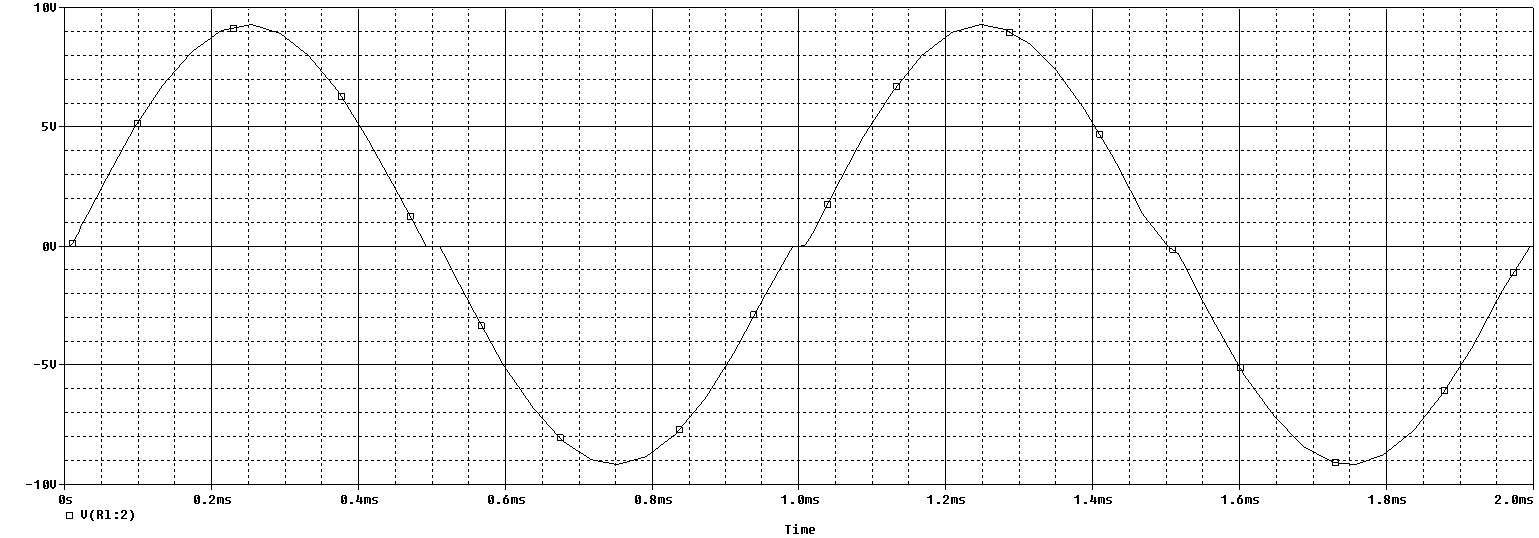
\includegraphics[width=1\textheight, angle=-90]{graf422V}
        \caption{Transitório da tensão de saída.}        
        \label{graf422V}
    \end{figure}
    
    \newpage
    
    \begin{figure}[h!] 
        \centering
        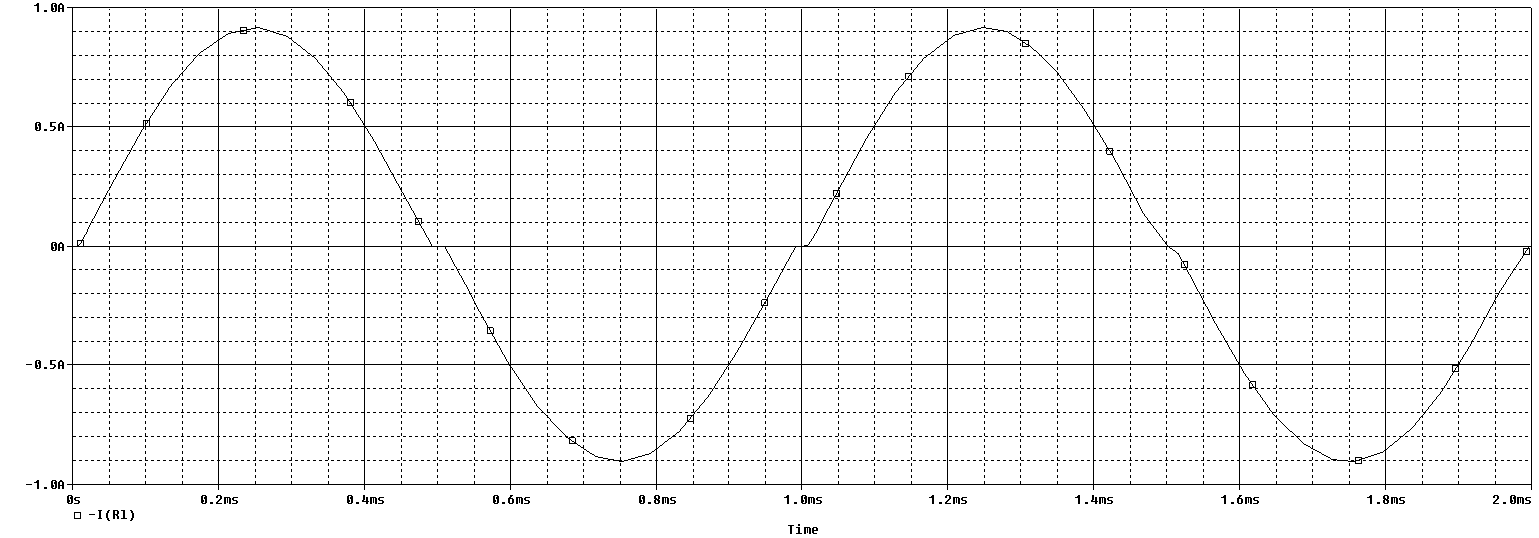
\includegraphics[width=1\textheight, angle=-90]{graf422I}
        \caption{Transitório da corrente de saída.}        
        \label{graf422I}
    \end{figure}
    
    \begin{figure}[h!] 
        \centering
        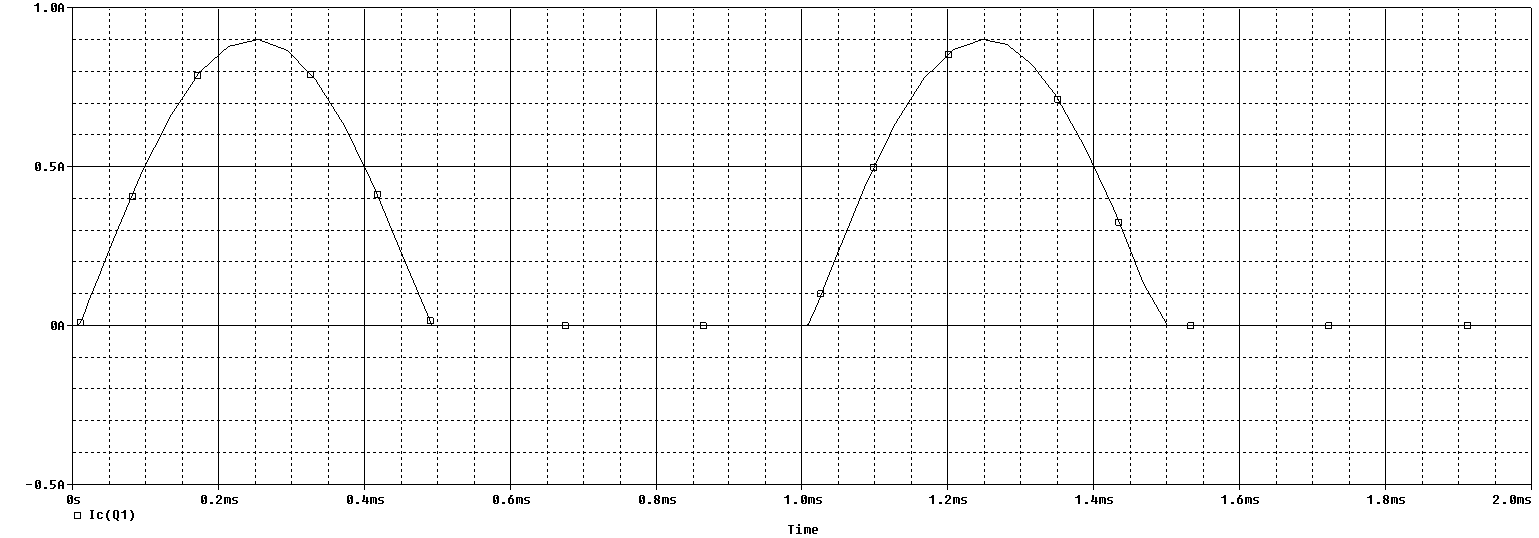
\includegraphics[width=1\textheight, angle=-90]{graf423I+}
        \caption{Transitório da corrente na fonte de tensão positiva
        \(V_{CC}\).}    
        \label{graf423I+}
    \end{figure}
    
    \newpage
    
    \begin{figure}[h!] 
        \centering
        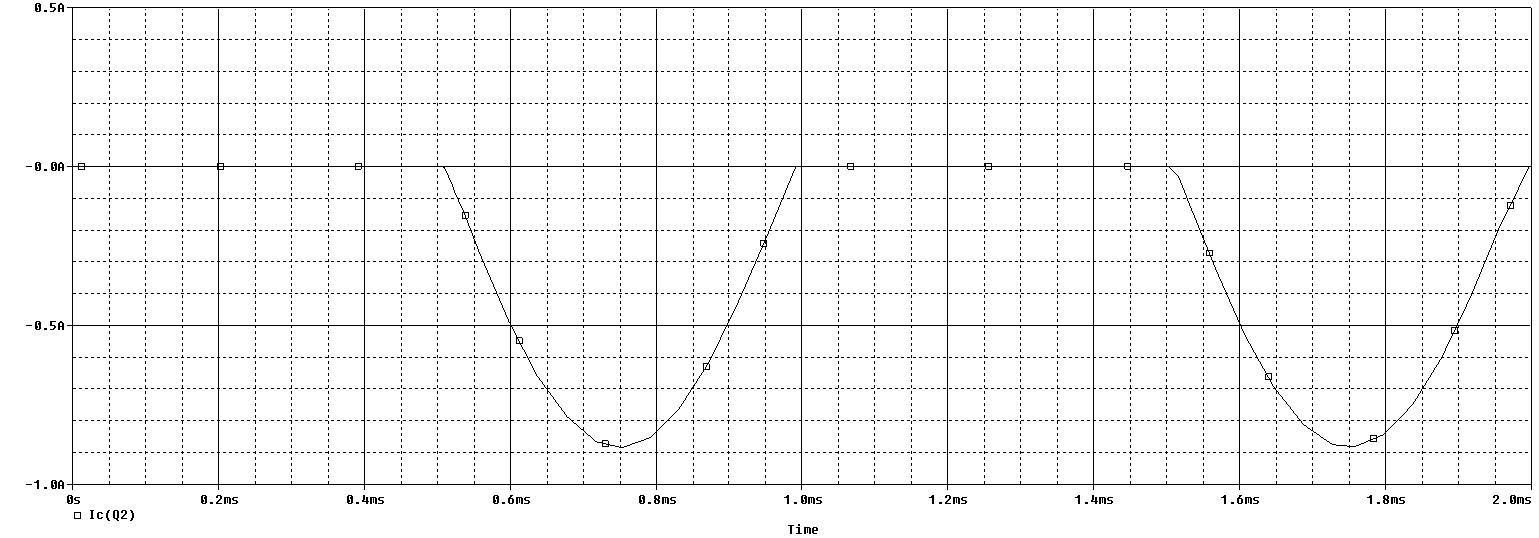
\includegraphics[width=1\textheight, angle=-90]{graf423I-}
        \caption{Transitório da corrente na fonte de tensão negativa \(-V_{CC}\).}        
        \label{graf423I-}
    \end{figure}
    
\end{document}